\section{Einige spezielle Graphen}
$K_n$: Vollständiger Graph nit $n$ Knoten (Clique)\\
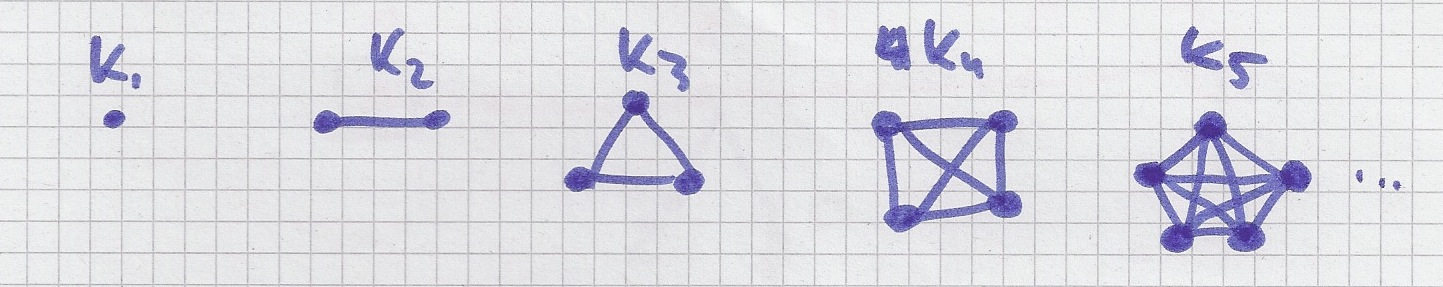
\includegraphics[width=\textwidth]{Bild44} \\
$C_n$: Kreis der Länge $n \:(n\geq 3)$\\
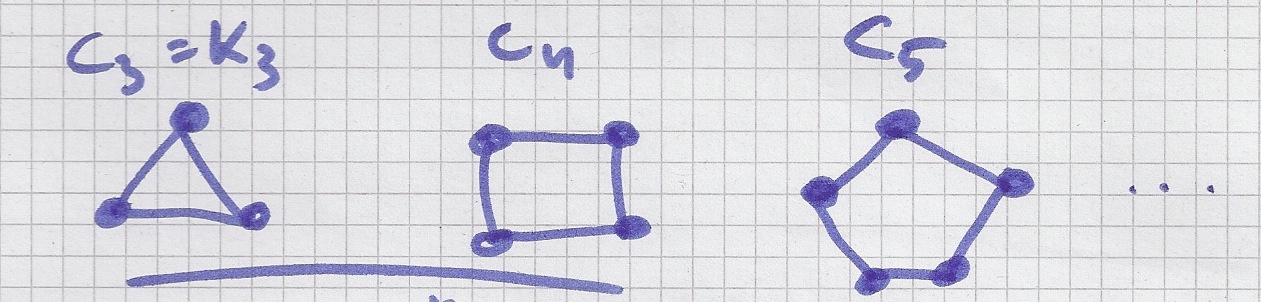
\includegraphics[width=\textwidth]{Bild45} \\
$M_{m,n}$\\
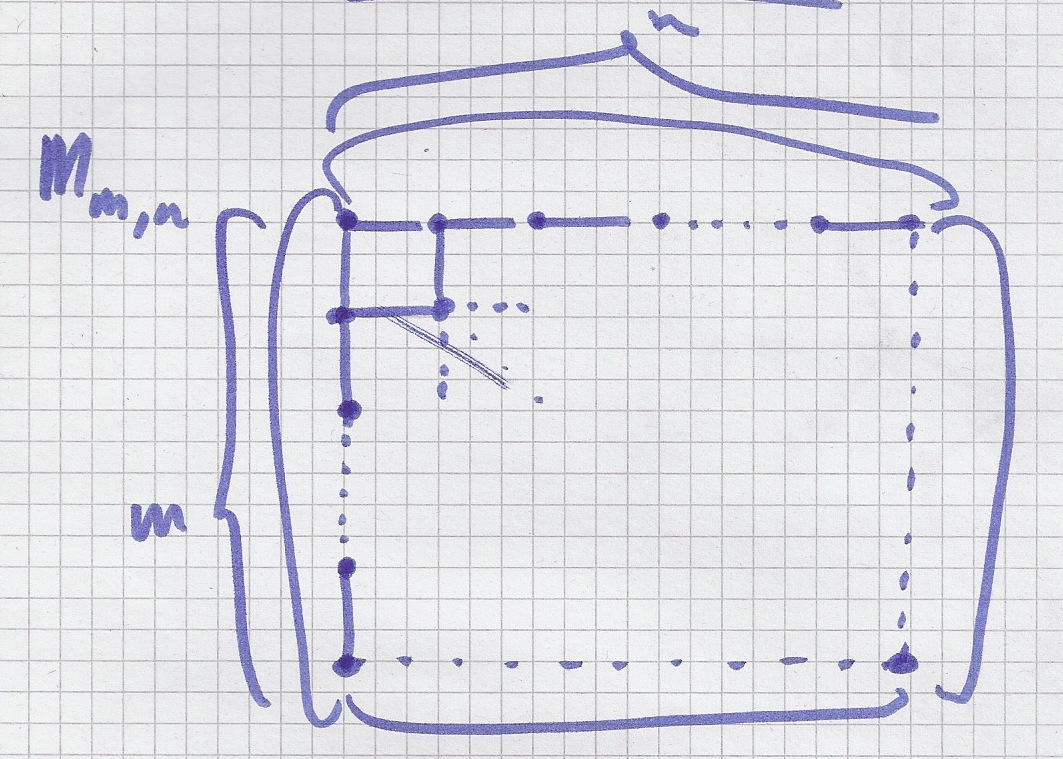
\includegraphics[width=\textwidth]{Bild46} \\
$V = \{ (i,j) : i = 1, \dotsc , m ; j = 1, \dotsc , n \}$\\
$\{(i,j),(i',j')\} \in E \iff \abs{i-i'} + \abs{j-j'} = 1$\\
zyklisch\\
$K_{m,n}$: Vollständiger bipartiter Graph (zwei-färbbar)\\
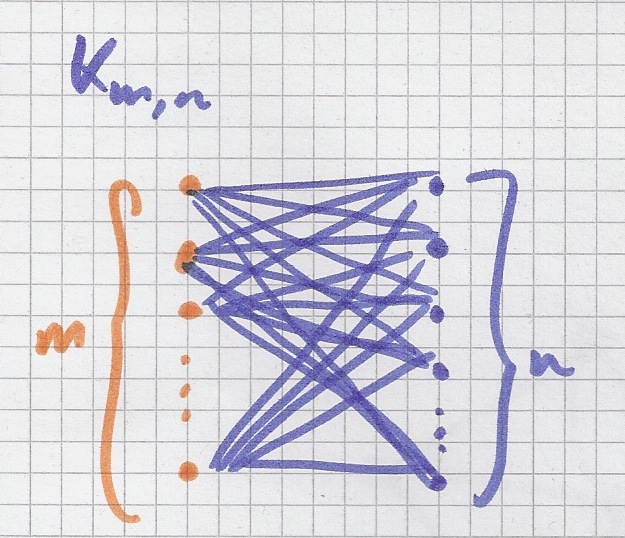
\includegraphics{Bild47} \\
$Q_d$: $d$-dimensionaler Hyperkubus \\
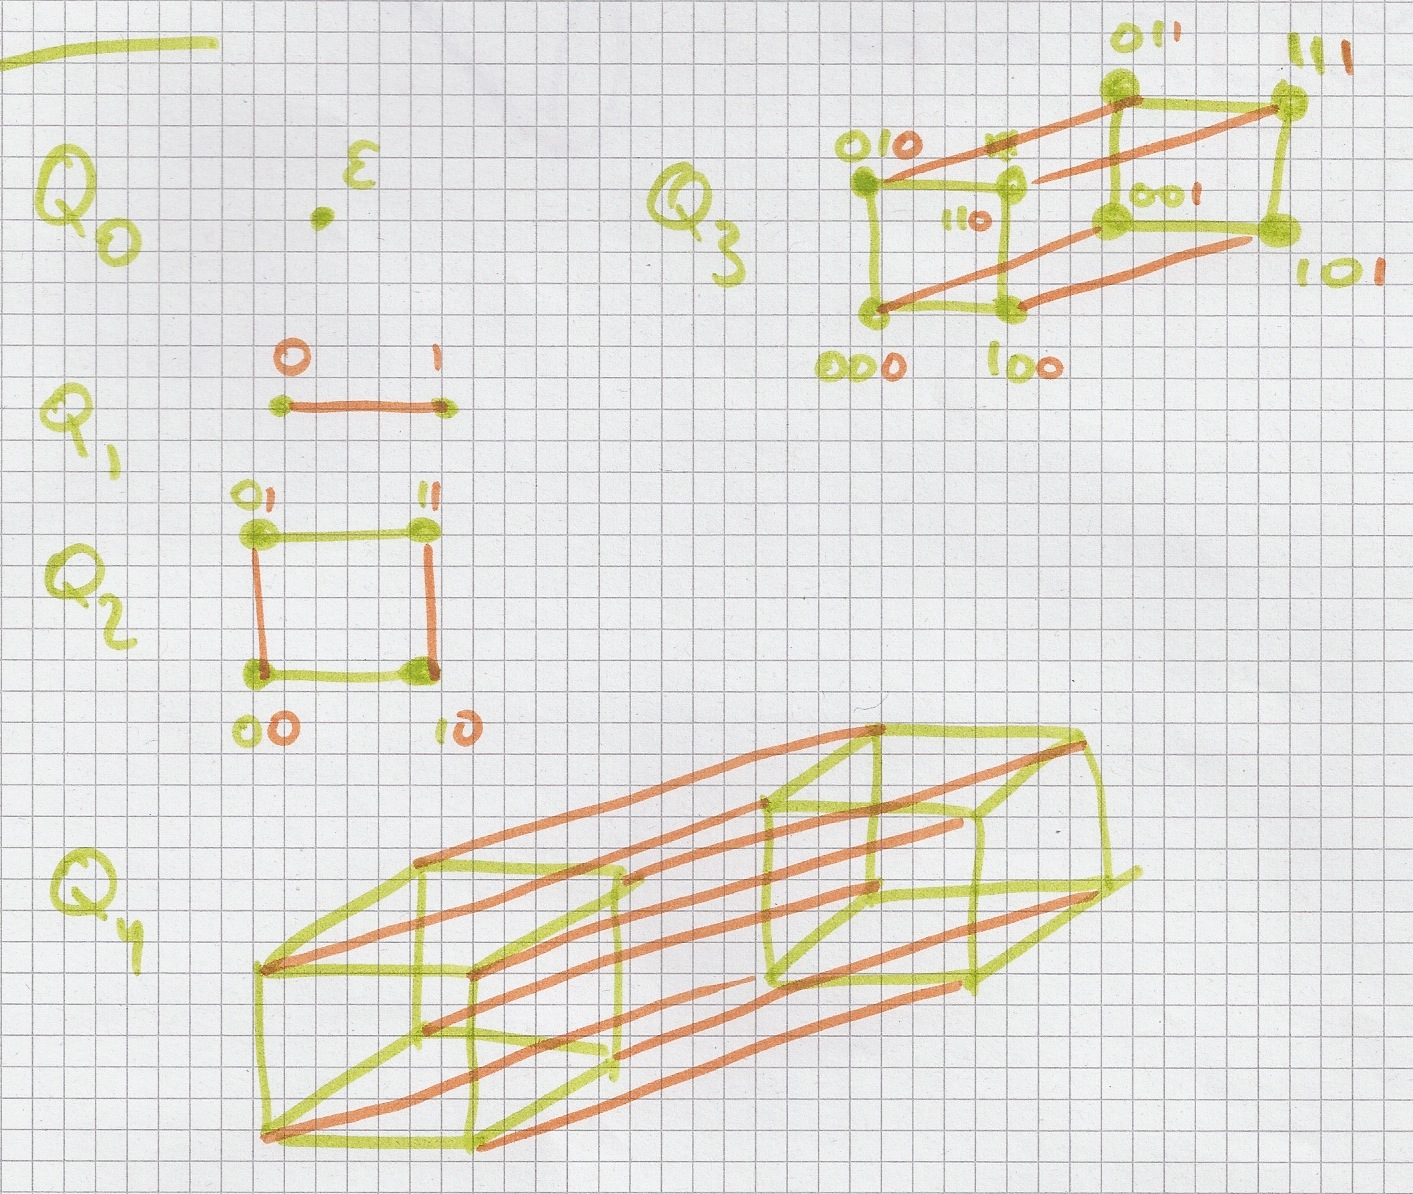
\includegraphics[width=\textwidth]{Bild48} \\
$V = \{ 0 , 1 \}^d$\\
$\{ u , v \} \in E :\iff d_H( u , v ) = 1$\\
$d_H$ \enquote{Hamming-Distanz}: Anzahl differenzierende Bit-Positionen\\
\begin{bsp*}
	\[ d_H( 0110110 , 1011010 ) = 4 \]
\end{bsp*}
\begin{gather*}
	\abs{V} = 2^d \\
	\abs{E} = \frac{\sum_{v \in E} \overbrace{\deg(v)}^{=d}}{2} = \frac{2^d \cdot d}{2} = 2^{d-1} \cdot d
\end{gather*}